\documentclass{sig-alternate}

%\documentclass{acm_proc_article-sp}
\usepackage{algorithmic}
\usepackage{algorithm}
\usepackage{graphicx}
\usepackage{url}
%\usepackage{amsmath}
%\usepackage{amsthm}
\usepackage[small,it]{caption}
\DeclareCaptionType{copyrightbox}
\usepackage{subcaption}
\newtheorem{theorem}{Theorem}
\newtheorem{lemma}{Lemma}
\newtheorem{corollary}{Corollary}
\newtheorem{proposition}{Proposition}
\newtheorem{definition}{Definition}
\begin{document}
%
% --- Author Metadata here ---
%\conferenceinfo{WOODSTOCK}{'97 El Paso, Texas USA}
% --- End of Author Metadata ---

\title{Adaptive Defending Strategy for Smart Grid Attacks}

% There's nothing stopping you putting the seventh, eighth, etc.
% author on the opening page (as the 'third row') but we ask,
% for aesthetic reasons that you place these 'additional authors'
% in the \additional authors block, viz.

% Just remember to make sure that the TOTAL number of authors
% is the number that will appear on the first page PLUS the
% number that will appear in the \additionalauthors section.
\numberofauthors{2} 

\author{
% You can go ahead and credit any number of authors here,
% e.g. one 'row of three' or two rows (consisting of one row of three
% and a second row of one, two or three).
%
% The command \alignauthor (no curly braces needed) should
% precede each author name, affiliation/snail-mail address and
% e-mail address. Additionally, tag each line of
% affiliation/address with \affaddr, and tag the
% e-mail address with \email.
%
% 1st. author
\alignauthor
Jianye Hao, Eunsuk Kang, \\Daniel Jackson\\
       \affaddr{Massachusetts Institute of Technology}\\
      \email{\{jianye, eskang, dnj\}@mit.edu}
% 2nd. author
% \alignauthor
% Eunsuk Kang\\
%        \affaddr{Massachusetts Institute of Technology}\\
%        \email{eskang@csail.mit.edu}
% % 3rd. author
% \alignauthor Daniel Jackson\\
%        \affaddr{Massachusetts Institute of Technology}\\
%        \email{dnj@mit.edu}
\and  % use '\and' if you need 'another row' of author names
% 4th. author
\alignauthor Jun Sun\\
       \affaddr{Singapore University of Technology and Design}\\
         \email{sunjun@sutd.edu.sg}
}

\maketitle
\begin{abstract}
One active area of research in smart grid security focuses on applying
game-theoretic frameworks to analyze interactions between a system and
an attacker and formulate effective defense strategies. In previous work,
a Nash equilibrium (NE) solution is chosen as the optimal defense
strategy \cite{law2012security,ma2013markov}, which implies that the
attacker has complete knowledge of the system and would also employ
the corresponding NE strategy. In practice, however, the attacker may
have limited knowledge and resources, and thus employ an attack which
is less than optimal, allowing the defender to devise more efficient
strategies.

We propose a novel approach called an \underline{a}daptive
\underline{M}arkov \underline{s}trategy (AMS) for defending a system
against attackers with unknown, dynamic behaviors. The algorithm for
computing an AMS is theoretically guaranteed to converge to a best
response strategy against any stationary attacker, and also converge
to a Nash equilibrium if the attacker is sufficiently intelligent to
employ the AMS to launch the attack. To evaluate the effectiveness of
an AMS in smart grid systems, we study a class of data integrity
attacks that involve injecting false voltage information into a
substation, with the goal of causing load shedding (and potentially a
blackout). Our preliminary results show that the amount of load
shedding costs can be significantly reduced by employing an AMS over
a NE strategy.

\end{abstract}

% A category with the (minimum) three required fields
%\category{H.4}{Information Systems Applications}{Miscellaneous}
%A category including the fourth, optional field follows...
%\category{D.2.8}{Software Engineering}{Metrics}[complexity measures, performance measures]

%\terms{Theory}

%\keywords{ACM proceedings, \LaTeX, text tagging}
\section{Introduction}

Power grid is one of the most critical infrastructures in existence today, whose disruption could cause severe economic, social, and environmental damages \cite{brown2006defending,salmeron2004analysis}, making it an attractive target for attackers. Protecting a power grid poses a number of challenges due to its wide geographical spread and complex interdependences among its components. To make the matter worse, modern grid systems are connected to the Internet, exposing itself to a wide range of cyber-attacks.

One active area of research in smart grid security focuses on applying game-theoretic frameworks to analyze the interactions between system defenders and attackers \cite{saad2012game}. One commonly adopted game-theoretic model is called a Markov game \cite{minmaxQ}, where the players' joint actions lead to probabilistic transitions between states of the system. In the previous applications of a Markov game to a smart grid attack, a \textit{Nash equilibrium} (NE) solution is computed as the optimal defending strategy \cite{law2012security,ma2013markov}. 

The proposal on adopting a NE strategy is based on one crucial assumption: the attacker would also employ the corresponding NE strategy to attack the system. In practice, for a system as complex as a smart grid, the attacker may have neither a perfect knowledge of the system nor the computational capacity required to compute a NE strategy. More realistically, the attacker uses its experience and partial knowledge of the system to formulate what he/she believes to be the best strategy for maximizing the damage. Thus, it may be possible for the defender to employ a non-NE strategy that is just as effective, and potentially cheaper. The technical challenge is determining the attacker's behavior (initially unknown) and reformulate the defender's strategy dynamically.

%This kind of analysis is usually based on the assumption that the attackers are strategic and individually rational in maximizing the possible cost incurred on the system. One commonly adopted game-theoretic model is the Stackelberg game, which models the strategic interaction among defender and attacker as a two-player single-shot sequential game. This kind of modeling is based on the assumption that the attacker has the capability to observe the protection strategy of the defender through extensive surveillance, which usually might not be feasible in practice.

We propose a novel approach called an \underline{a}daptive \underline{M}arkov \underline{s}trategy (AMS) for defending a system against attackers with \emph{unknown, dynamic} behaviors. Our AMS algorithm leverages an adaptive online learning technique to observe the attacker's behavior and reformulate an optimal defense strategy dynamically. It is guaranteed to converge to a best-response strategy against any stationary attacker, and also converges to a Nash equilibrium if the attacker is sufficiently intelligent to employ the AMS to launch the attack.

To demonstrate the effectiveness of our approach, we applied it to a class of smart grid attacks that involve injecting false voltage information into a grid substation, disrupting its voltage stability and causing load shedding. We experimentally evaluated the performance of our approach by applying it to a sample distribution system from the previous work \cite{law2012security}. Our preliminary results show that the amount of load shedding cost can be significantly reduced by employing an AMS over a NE strategy. Although we focus on one particular type of security attacks in this paper, our learning framework is general, and applicable to other classes of attacks that can be modeled as a Markov game.

The rest of the paper is organized as follows. We give an overview of related work in Section \ref{relatedwork}. In Section \ref{problemdefinition}, we describe the false data injection attack and how this problem can be modeled as a Markov game. We present the AMS strategy and its properties in Section \ref{amsstrategy}, and describe an evaluation of our approach in Section \ref{simulation}. We conclude with a discussion of future work in Section \ref{conclusion}.



\section{Related Work}
\label{relatedwork}
Game theory has been widely used as a mathematical tool to model and analyse the security issues in critical infrastructures such as smart-grid systems \cite{saad2012game,brown2006defending,salmeron2004analysis,pinar2010optimization}. The interaction between the defender and attacker is usually modeled as a single-shot Stackelberg game, in which the defender and attacker are considered as the leader and follower and make sequential moves. The goal thus is to identify the optimal defending strategy (e.g., the most critical set of components to protect) for the defender to minimize the potential loss of the system. However, in practice the defender and attacker may interact with each other repeatedly and the system evolves dynamically depending on their actions.

Markov games \cite{minmaxQ} later are adopted to model the repeated strategic interactions between the defender and attacker in smart-grid systems. In \cite{ma2013markov}, one specific physical attack on the transmission lines of the smart-grid system is considered and the interaction between the defender and attacker is modeled as a Markov game, in which the system states (the status of the transmission lines) evolves based on their joint actions. A NE solution is adopted as the defending strategy for the system, which specifies which transmission lines to protect. In \cite{law2012security}, one specific cyber attack (false data injection attack) is studied and the repeated attacker-defender cyber-interaction is modeled as a Markov game. Similar to \cite{ma2013markov}, the NE solution is adopted as the defending strategy which determines which action to choose to perform intrusion detection. However, adopting the NE solution as the defending strategy is rational only when the attacker is also choosing the corresponding NE strategy to launch the attack, which may not hold in practice.



\section{Problem Formulation}
\label{problemdefinition}
\subsection{Threat Model}
\label{threatmodel}

\begin{figure}[t]
\setlength{\belowcaptionskip}{-15pt}
\centering
\captionsetup[subfigure]{aboveskip=-0.5pt,belowskip=-5pt}
 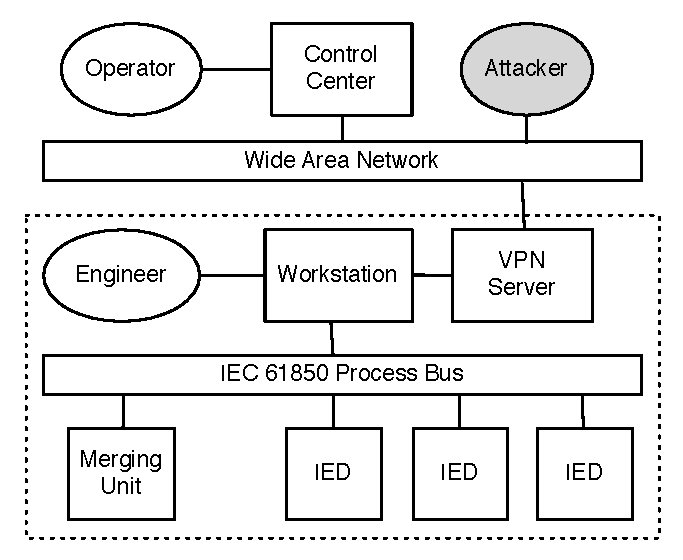
\includegraphics[width=0.6\columnwidth]{figures/substation-outline}
\caption{\scriptsize{A high-level architecture of a smart grid. The dotted area
  represents a substation.}}
 \label{fig:substation}
\end{figure}

One important requirement of a power grid is maintaining
a stable supply of voltage throughout its distribution and transmission
lines. Since many modern grids operate close to their stability
limits, even slight instability or disruption can cause the voltage to
drop below a critical level, forcing load sheddings and in the worst
cast, blackouts. In order to maintain stability, each substation
deploys a number of devices that monitor the voltage level and
dynamically regulate power. A typical high-level architecture of a
smart grid system is shown in Figure~\ref{fig:substation}, with the
dotted box representing one of its substations. A \textit{merging
  unit} collects various analog data from physical sensors (such as
voltage and current levels) and converts them into digital packets,
which are then broadcast over the process bus. A number of intelligent
electronic devices (IEDs), connected to the process bus, look for
anomalous readings in the packets and perform necessary regulating
actions. A \textit{static synchronous compensator} (STATCOM) is one
common type of device for voltage regulation, generating (absorbing)
power when notified of low (high) voltage in the load.

Many modern substations allow engineers to perform maintenance
remotely through a virtual private network (VPN) or other access
mechanisms. While convenient, this also opens up the substation to a
wide range of security attacks, since anyone on the Internet, having
bypassed the VPN, may manipulate various devices through the
workstation.

In this paper, we focus on one particular type of smart grid attacks
and corresponding defense mechanisms, orignally proposed in
\cite{law2012security}.

\noindent\textbf{Attack} We consider scenarios in which the attacker has
successfully gained access to the workstation by exploiting weakness
in its network perimeter (e.g., misconfigured firewall, weak
password/keys). We assume that the attacker wishes to
remain undetected, and so chooses not to perform drastic actions such
as shutting down the entire substation. Finally, we assume that the
attacker is not capable of physically tampering with the substation
components (e.g., tripping transmission lines using circuit breakers).

We focus on one class of attacks where an attacker manipulates the
behavior of a voltage regulator by injecting false voltage data into
the process bus~\cite{law2012security}. From the attacker's point of
view, this attack is particularly appealing since it can be carried
out in a stealthy manner; by injecting a stream of packets with small
deviations from normal voltage, the attacks may remain undetected by
the system until it results in a catastrophic result (i.e., a
blackout), similar to the way Stuxnet~\cite{farwell2011stuxnet} was
carried out.

In particular, given the actual voltage $v$, the attacker constructs a
packet that indicates a voltage value of $kv$, where $k$ is a constant
multiplicative factor. A STATCOM, having received the false
measurement, may unnecessarily inject (possibly causing overvoltage)
or absorb power from the load (under-voltage). When the actual voltage
drops below a certain level, this results in a load shedding enforced
by undervoltage load shedding relay \cite{lefebvre2004undervoltage}.

\noindent\textbf{Defense} One common mitigation against this type of attack
is the use of encryption to ensure the integrity of the
packets. However, relying on encryption as the sole protection
mechanism may not be sufficient for two reasons:
(1) a smart grid system has real-time requirements, with each packet
being sent and processed in a span of milliseconds, and so resources
required to encrypt and decrypt every packet may be too stringent, and
(2) encryption keys are often stored as part of a configuration file,
which may be easy to obtain once the attacker gains the entry to the
workstation. 

% A hardware-based encryption mechanism may address these
% issues, but they are still not common among IEDs, and so we do not
% discuss it in this paper.

Instead, we consider a threshold-based method for detecting bad data
packets \cite{law2012security}. In this method, the IED allocates an
internal variable to keep track of the number of times $I - I_{ref}$
deviates from 0, where $I$ is the current flowing through the current
generator in the IED, and $I_{ref}$ is a fixed reference current. If
this number exceeds some predefined threshold (frequency variable $\tau$) over a certain time
period, then the IED concludes that the
system may be under attack. The intuition behind this detection method
is that $I - I_{ref}$ should remain close to 0 under normal
circumstances, and that even in an unstable environment, should not
vary no more frequently than $\tau$. The best value for $\tau$ for detecting the cyber-attack varies depending on the specific range of the false voltage data injected by the attacker. Thus the challenge for the defender is to determine the right value for $\tau$ to maximize the detection success rate in response to the changes of the attacker's behaviors. We can adopt Markov game model to analyze this kind of strategic interaction between the defender and attacker, which will be described in the next section.
 
\subsection{Markov Games}

A Markov game is played between two players---the \textit{attacker}
and the \textit{defender}---over a possibly infinite sequence of
\textit{rounds}. During each round, both players perform an
\textit{action} that may cause changes to the state of the system with
some probabilities. Each player receives a corresponding payoff after
selecting an action simultaneously. In our case, since the goal of the
attacker is to trigger load shedding through false data injection
attack, the attacker's payoff may be measured by the amount of load
shedding that its action causes to a grid given the action of the
defender. Conversely, the payoff for the defender is the negation of
the amount of load shedding. The Markov game here is
\textit{zero-sum}; that is, the sum of the attacker's and defender's
payoffs is zero.

Formally, a Markov game consists of:
\begin{itemize}
\item $N$: a finite number of players. In our setting, there are two players (defender and attacker), i.e., $N = \{d, a\}$.
\item $A_i$: the action space of each player. $A_d$ and $A_a$ represent the set of defender's and attacker's actions, respectively. 
\item $S$: a finite set of system states. 
\item $Pr$: transition probability function. Given the current state
  $s$ and the joint action $(d, a)$, $Pr(d, a, s, s^\prime)$ returns the probability that the system transits
  from state $s$ to $s^\prime$ when the defender and the attacker perform
  actions $d$ and $a$, respectively.
\item $R_i$: payoff function of the players. Given $s \in S$, $a \in A_a$, and $d \in
  A_d$, $R_d(s, d, a)$ returns the expected payoff of the
  attacker when the joint action $(d, a)$ is performed under state $s$. Since we are
  interested in zero-sum games, the attacker's corresponding payoff $R_a(s, d, a)$ is exactly the negation of $R_d(s, d, a)$, i.e., $R_a(s, d, a) =  - R_d(s, d, a)$.
\end{itemize}

The behaviors of the attacker and defender from
Section~\ref{threatmodel} can be modeled as follows. First, the action
space of the attacker can be defined as
\begin{equation}
A_a = \{ k_1, k_2, ..., k_{N_a} \}
\end{equation}
where $k_1, k_2,...$ are real constants, $N_a$ is the size of $A_a$,
and for some $i \leq N_a$, $k_i$ corresponds to the injection of a
packet that indicates a voltage level of $k_{i}b$ (i.e., falsely
magnifying the voltage reading by a factor of $k_{i}$).

Similarly, the set of the actions that the defender may
perform is defined as:
\begin{equation}
A_d = \{ \tau_1, \tau_2, ..., \tau_{N_d} \}
\end{equation}
where $\tau_1, \tau_2, ...$ are integer constants, $N_d$ is the size
of $A_D$, and for some $j \leq N_d$, $\tau_j$ refers to the
defender deploying the detection method with the threshold of
$\tau_j$ (i.e., the number of times $I - I_{ref}$ is allowed to cross 0). 

A player's \textit{strategy} $\phi$ is a function that given some
state $s$, returns a probability distribution over the set of actions
that the player may perform in $s$.


%describe the game-theoretic modeling of the defender-attacker model (refer to \cite{ma2013markov}). The difference is that we assume that each time the attacker launchs an attack on the system and the system's performance is degraded due to the attack, the system will be restored to its initial state before the next attack occurs (any damaged transimission link will be repaired). In this way, the origianl markov game model can be reduced to the repeated game model- markov game with only one state.

\section{Adaptive Protection}
\label{amsstrategy}
In the previous section, we have shown how we can model a security attack as a Markov game between the attacker and the defender. From the system architect, one important question is how the system should choose its defending strategy in order to minimize the amount of damage caused by the attacker. A conventional approach in the game theory is computing a \textit{Nash equilibrium} (NE) strategy: that is, both the attacker and the defender play a strategy that would maximize the payoffs for both of them \cite{law2012security, ma2013markov}. The rationale for adopting the NE solution is that neither the attacker nor the defender can do better by choosing a different strategy.

However, in practice, choosing a NE strategy is not necessarily optimal for the defender, since it depends on a number of assumptions that might not hold. First, computing a NE relies on a perfect knowledge of the system; however, in reality, the attacker might not have the capability to collect enough information to construct an accurate model of a smart grid. Second, since the attackers are humans, it is likely that they would launch attacks based on their intuition or past experience, which might be different from the NE strategy. Lastly, if there are multiple equilibria, the players may not pick the same matching strategy.

Instead, an effective defending strategy should be \textit{adaptive}, i.e., it should be able to learn the attacker's strategy and dynamically compute the \textit{best response} strategy to counter the attacking strategy. However, assuming that the attacker may change its strategy arbitrarily is neither useful nor practical. Therefore, to make our technique feasible, we assume that the attacker's strategy is \textit{stationary} (i.e., the probability of choosing each action is unchanged under the same state)\footnote{We allow the attacker to change its strategy to another stationary strategy during the game.}.

An effective defending strategy must satisfy the following two desirable properties \cite{bowling2001convergence}.

\begin{description}
\item[Rationality] A \emph{rational} defending strategy must always learn to play the best response strategy given that the attacker is adopting a stationary attacking strategy. Satisfying this property guarantees that the cost to the system can be minimized as long as the attacker's strategy is stationary. Note that a NE strategy is a special case of stationary strategy.

\item[Convergence] The defending strategy must always converge to a stationary strategy under self-play.  This property takes into consideration the possibility that the attacker might be as intelligent as the defender and employ the same adaptive strategy as the defender. We can see that under self-play, if both rationality and convergence properties are satisfied, the defender and attacker will eventually converge to a NE strategy. This means that the maximum cost to the system can be bounded to the cost when the attacker adopts a NE strategy, even when the attacker is as intelligent as the defender.
\end{description}

\subsection{AMS: Adaptive Markov Strategy}

In this section, we propose an algorithm for computing an \underline{a}daptive \underline{M}arkov \underline{s}trategy (AMS) for defending a system against security attacks. Our algorithm is based on the AWESOME algorithm~\cite{conitzer2007awesome}, which computes adaptive defending strategies for repeated games only (i.e., a special case of Markov games where the system has exactly one state); we extend AWESOME to Markov games where the system may have any finite number of states.  

Before introducing the AMS algorithm in details, we need to explain a few terms first. First, to determine whether the attacker is employing the NE or any other stationary strategies, we define the \emph{distance} between two strategies to compare whether they are the same or not. 

\begin{definition}
The \emph{distance} $Distance(\phi_1, \phi_2)$ between two stationary strategy $\phi_1$ and $\phi_2$ is: 
\begin{equation}
Distance(\phi_1, \phi_2) = \max|\phi_1(s,a) - \phi_2(s,a)|, \forall a\in A_s, s\in S
\end{equation}
where $A_s$ is the action space at state $s$ and $S$ is the state space, and $\phi_1(s,a)$ and $\phi_2(s,a)$ is the probability that action $a$ is played at state $s$ for strategy $\phi_1$ and $\phi_2$ respectively.
\end{definition}

Second, given two strategies $\phi_1$ and $\phi_2$, we define the value $V(s, \phi_1, \phi_2)$ of playing strategy $\phi_1$ against strategy $\phi_2$ under state $s$, which is defined as the sum of the discounted expected payoff obtained over infinite number of interactions.
\begin{definition}
\label{valueofstate}
The value $V(s, \phi_1, \phi_2)$ of playing strategy $\phi_1$ against strategy $\phi_2$ under state $s$ is defined as follows, 
\begin{equation}
\begin{split}
V(s, \phi_1, \phi_2) = &R(s, \phi_1(s), \phi_2(s)) +\\& \delta\sum_{s\in S} Pr(\phi_1(s), \phi_2(s), s, s^\prime)V(s^\prime, \phi_1, \phi_2)
\end{split}
\end{equation}
\end{definition}
where $\delta$ is the discounting factor reflecting the relative importance of future payoffs and $Pr(\phi_1(s), \phi_2(s), s, s^\prime)$ is the probability that the system state transits from $s$ to $s^\prime$ given that the players choose actions $\phi_1(s)$ and $\phi_2(s)$ respectively. We can construct one equation for V-value of each state $s\in S$ following Definition \ref{valueofstate}, and thus the value of each state can be calculated by solving the system of $|S|$ linear equations using different techniques such as iterative methods \cite{eisenstat1983variational}.

The AMS algorithm (Algorithm \ref{AMS}) takes place over consecutive \textit{periods} (where each period is some number of round)\footnote{Each round of attacker-defender interaction might take a few minutes in the smart-grid system.}. Initially, the AMS begins by playing the precomputed NE strategy\footnote{We only need to compute the minmax strategy instead since for a zero-sum Markov game, the minmax/maxmin strategy for each player is equivalent with its corresponding NE strategy \cite{sigaud2013markov}. Generalized value iteration algorithm \cite{sigaud2013markov} can be used to compute the minmax strategy efficiently and we omit the details due to space limitation.} for the initial period $N^0$ (Line 5) and estimates the strategy of the attacker based on the actions taken in this period (Line 7 to 10). If the \emph{distance} between the estimated strategy $h_a^{curr}$ and the NE strategy $\pi_a^*$ of the attacker is larger than the given threshold (line 13), the attacker is considered playing a non-NE strategy, and a random strategy is chosen as the defense strategy for the next period (Line 17). 

\begin{algorithm}[t]\small
\caption{Description of AMS}
\label{AMS}
\begin{algorithmic}[1]
\STATE Compute NE strategy ($\pi^*_i, \forall i\in\{d,a\}$)
\REPEAT 
\STATE Initialize $h_a^{prev}$, $h_a^{curr}$ to nil
\STATE $s = s_0$, $\beta = false$, $t = 0$
\STATE Set defender strategy $\phi_d$ as NE strategy ($\phi_d = \pi_d^*$)
\WHILE{true}
\FOR{$r$ : 0 \TO  $N^t$}
\STATE Play($\phi_d(s)$)
\STATE Update($h_a^{curr}$)
\ENDFOR
\STATE $h_a^{prev} = h_a^{curr}$
\STATE $t$ := $t + 1$

     \IF{Distance($h_a^{curr}$, $\pi_a^*$) > $\epsilon^t_e$}
     \STATE  \textbf{break}
      \ENDIF
\ENDWHILE

\STATE $\phi_d$ = RandomStrategy()
\WHILE{true}
\FOR{$r$ : 0 \TO  $N^t$}
\STATE Play($\phi_d(s)$)
\STATE Update($h_a^{curr}, h_a^{prev}$)
\ENDFOR
\STATE $t$ := $t + 1$

  \IF{$\beta$ = true}
     \IF{Distance($h_a^{curr}$, $h_a^{prev}$) > $\epsilon^t_s$}
        \STATE \textbf{break}
      \ENDIF
  \ENDIF
  \STATE $h_a^{prev} = h_a^{curr}$
   \STATE $\beta := true$
   \STATE $\phi_d^\prime$ := BestResponseStrategy($h_a^{curr}$)
   \IF{$V(s,\phi_d^\prime, h_a^{curr}) > V(s,\phi_d, h_a^{curr}) + 2|A|^{|S|}\epsilon^{t+1}_s\mu$, $\forall s \in S$}
       \STATE $\phi_d = \phi_d^\prime$
   \ENDIF
\ENDWHILE
\UNTIL{}
\end{algorithmic}
\end{algorithm}

At the end of the next period, AMS computes the best response strategy $\phi_d^\prime$  against the current estimated strategy $h_a^{curr}$ of the attacker based on the last period's interaction (Line 31).\footnote{Generalized value iteration algorithm can be adopted here to compute the best response strategy in a Markov game \cite{sigaud2013markov}, and we skip the details due to space limitation.} If for every state $s\in S$, the difference between the V-value of $\phi_d^\prime$ against the $h_a^{curr}$ and that of $\phi_d$ is larger than the given threshold $2|A|^{|S|}\epsilon^{t+1}_s\mu$ (where $|A|^{|S|}$ represents the total number of pure strategies of the Markov game and $\mu$ is the payoff difference between the AMS player's best and worse outcomes), the current defending strategy $\phi_d$ is replaced by a more optimal strategy $\phi_d^\prime$ (Line 32-34).


\begin{figure*}[t]
\setlength{\belowcaptionskip}{-10pt}
\centering
 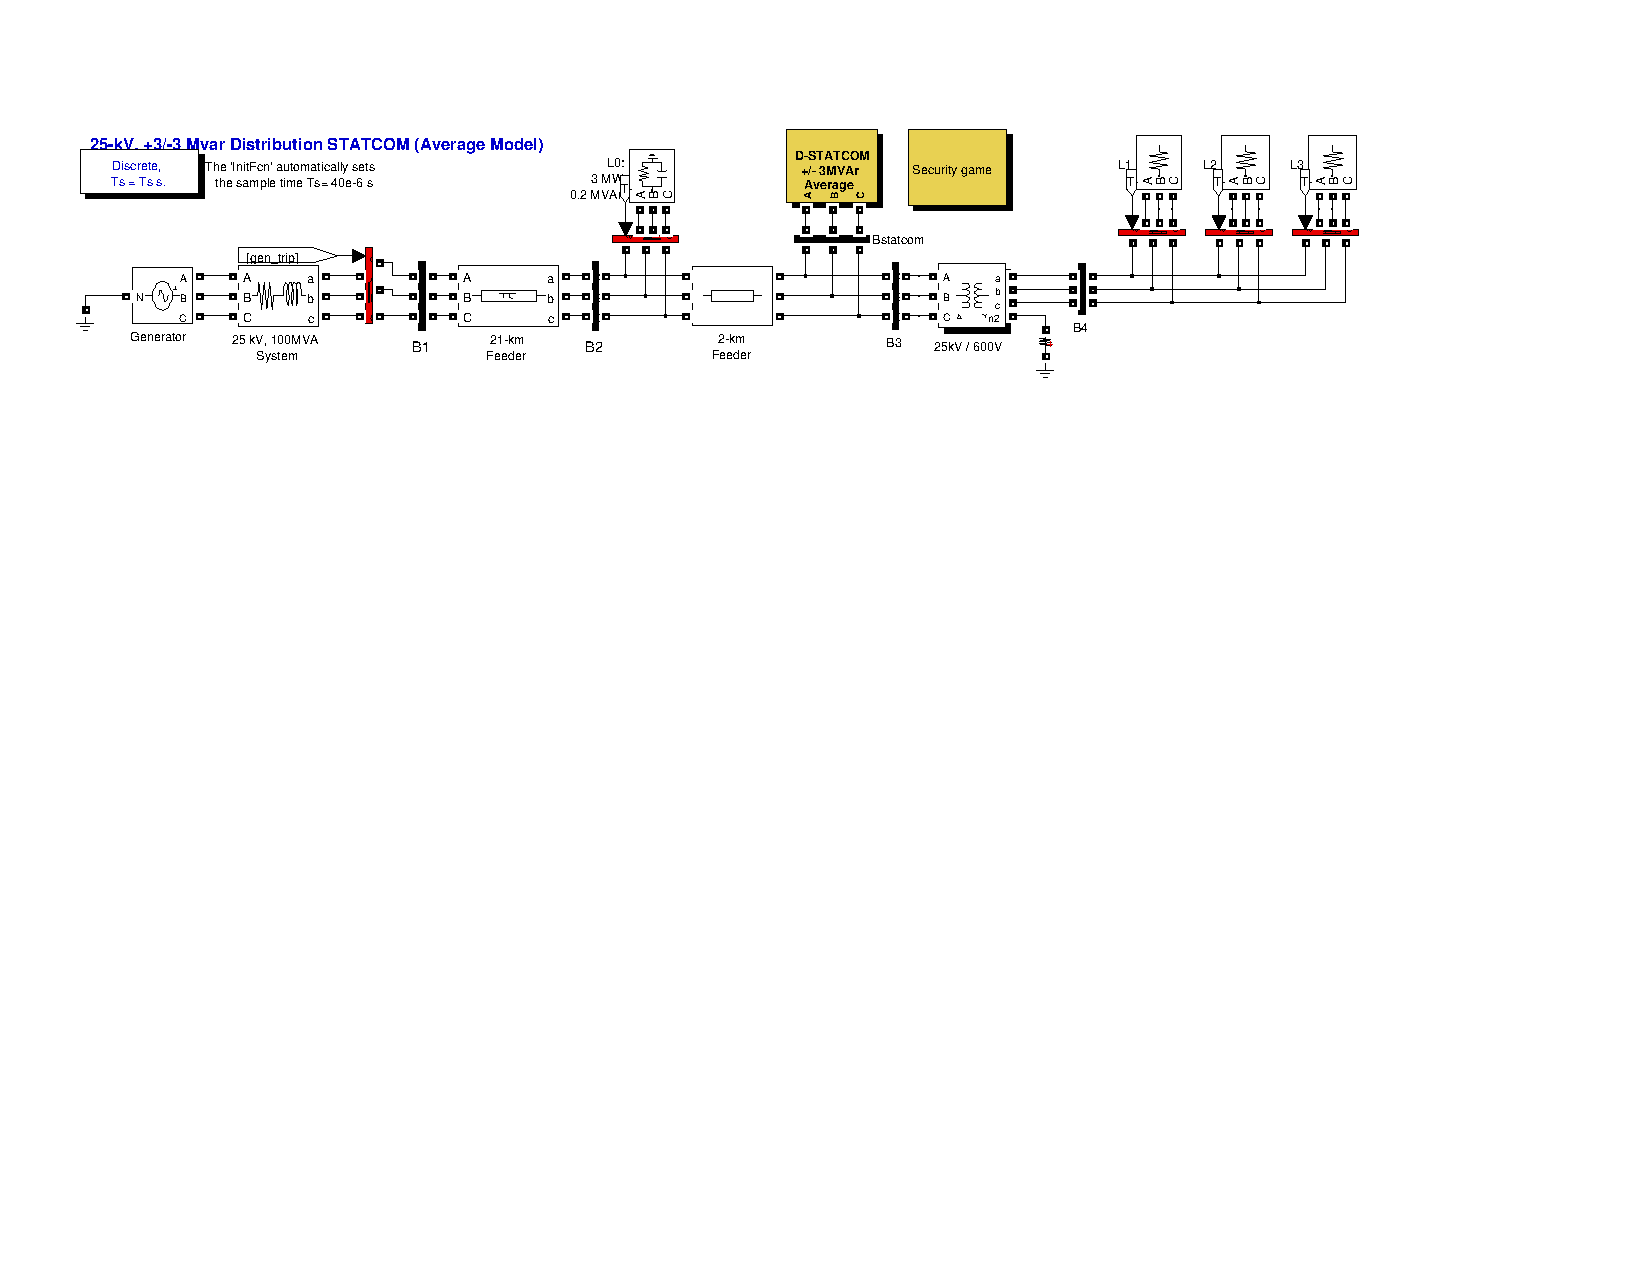
\includegraphics[width=0.95\textwidth]{example}
\caption{\scriptsize{An example distribution system with 1 generator and 4 buses \cite{law2012security}, originally from the D-STATCOM model in SimPowerSystems~\cite{simpowersystems}.}}
 \label{fig:example}
\end{figure*}

At the end of each following period, AMS compares the estimated strategy $h_a^{curr}$ and $h_a^{prev}$ of the attacker in the last and preceding periods (Line 25). If the distance between these two is larger than the given threshold $\epsilon_s^t$, it indicates that the opponent is not playing according to the estimated strategy $h_a^{prev}$, and the AMS will restart by breaking from the second while loop (Line 26). Otherwise, the AMS computes a best response strategy $\phi_d^\prime$ based on the last period's interaction, and employs $\phi_d^\prime$ as its strategy if it is more optimal than $\phi_d$ (Line 31-34). This process repeats as indicated by the outer \emph{Repeat} loop. 

The remaining question is how the set of parameters of the AMS algorithm should be adjusted, described as follows.

\begin{definition}
A schedule of adjusting the parameters \\$\{\epsilon_e^t, \epsilon_s^t, N^t\}$ is valid if
\begin{itemize}
\item $\epsilon_e^t, \epsilon_s^t$ are decreased monotonically and converge to zero eventually.
\item the value of $N^t$ is increased monotonically to infinity.
\item $\Pi_{t\in\{1,2,\ldots\}}(1 - A_S\frac{1}{N^t(\epsilon_s^{t+1})^2}) > 0$, where $A_S$ is the total number of actions of the defender summed over all states.
\end{itemize}
\end{definition}

\subsection{Properties of the AMS}

As previously mentioned, an effective defending strategy must satisfy two desirable properties: rationality and convergence. It can be theoretically proved that the AMS satisfies both properties, which are formalized as the following two theorems: 

\begin{theorem}
\label{rationality}
Given a valid schedule of adjusting the parameters, if the attacker employs a stationary attacking strategy, the defender adopting AMS eventually converges to a best response to the attacker's strategy with probability one.
\begin{proof}
We only provide a sketch of the proof here due to limited space. This theorem can be proved by dividing it into two parts. First, we prove that with non-zero probability, the AMS will never restart. We can show that the joint probability that the AMS will not restart for every period $t$ is greater than zero based on the triangle inequality and Chevyshev's inequality theorem. 

Second, we prove that the probability that the AMS never restarts and does not converge to a best response strategy against the attacker is 0 by continuity and Chevyshev's inequality theorem.  By proving both parts, we can conclude that the AMS will converge to a best response strategy against the attacker with probability 1.
\end{proof}
\end{theorem}

\begin{theorem}
\label{convergence}
Given a valid schedule, if both the defender and attacker employ the AMS, they eventually converge to a NE with probability one.
\begin{proof}
This theorem can be proved in a similar way to Theorem \ref{rationality}, and we omit the details due to limited space.
\end{proof}
\end{theorem}

\section{Experimental Simulation}
\label{simulation}

In this section, we describe a preliminary evaluation of the performance of an AMS for defending a substation against false data injection. We used a model of 1-generator 4-bus distribution system shown in Figure \ref{fig:example} (adopted from \cite{law2012security}) as the testbed, and compared the AMS's performance with that of the NE strategy proposed in \cite{law2012security,ma2013markov}. In this distribution system, the generator supplies electric power to four loads, and one STATCOM, connected to the system through Bus 3 (B3), regulates the voltage level by injecting (absorbing) reactive power to the system based on voltage feedback.
% As discussed in Section \ref{threatmodel}, the attacker intrudes the system and sends false voltage information back to the STATCOM, which might result in under-voltage and, eventually, load shedding. For the defender to protect against this kind of attack, certain detection algorithm can be implemented on the side of the STATCOM and the meter will be disconnected from the STATCOM if it detects that the meter has been compromised.

\begin{figure*}[t]
\setlength{\belowcaptionskip}{-12pt}
  \centering
\captionsetup[subfigure]{aboveskip=-1pt,belowskip=-7pt}~\hspace{-6em}
 \begin{subfigure}[b]{0.3\textwidth}
   \centering
                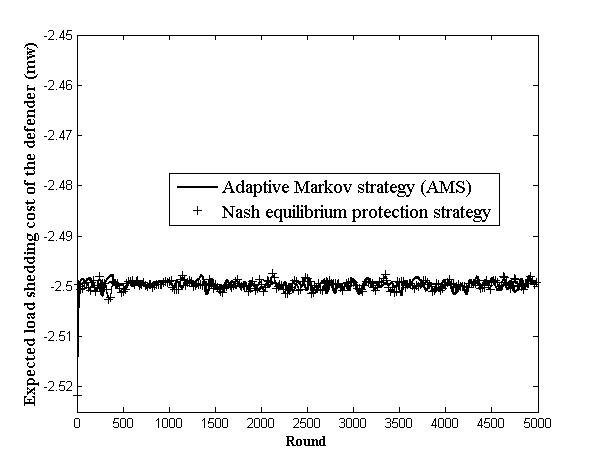
\includegraphics[width=1.4in]{result2}
                \caption{$\phi_0$: the NE strategy}
                \label{fig:NE}
        \end{subfigure}~\hspace{-6em}
 \begin{subfigure}[b]{0.3\textwidth}
   \centering
                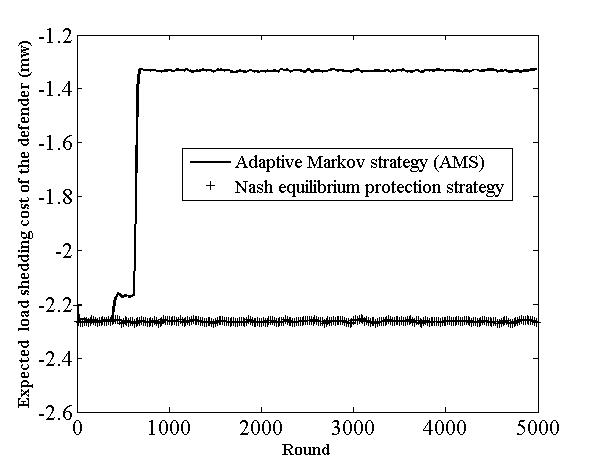
\includegraphics[width=1.4in]{result1}
                \caption{$\phi_1(s_1)  = \phi_1(s_2) = a _1$}
                \label{fig:a1}
        \end{subfigure}~\hspace{-6em}
\begin{subfigure}[b]{0.3\textwidth}
  \centering
                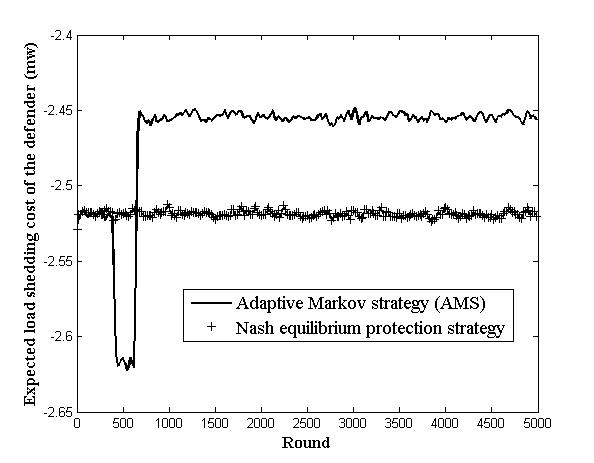
\includegraphics[width=1.4in]{result3}
                \caption{$\phi_2(s_1)  = \phi_2(s_2) = a _2$}
                \label{fig:a2}
        \end{subfigure}~\hspace{-4em}
\begin{subfigure}[b]{0.3\textwidth}
  \centering
                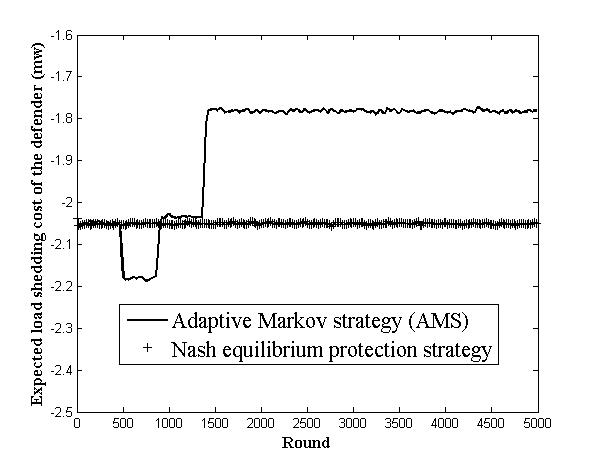
\includegraphics[width=1.4in]{result4}
                \caption{$\phi_3$: choose $a_1/a_2$ randomly}
                \label{fig:a1a2}
        \end{subfigure}~\hspace{-3em}
\begin{subfigure}[b]{0.3\textwidth}
  \centering
                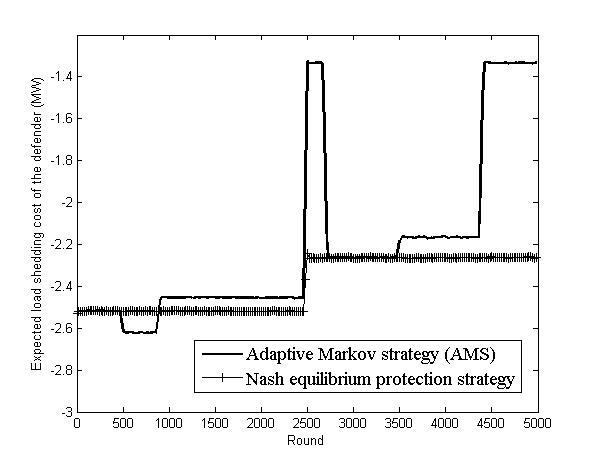
\includegraphics[width=1.4in]{result5}
                \caption{0 - 2500:$\phi_2$, 2500 - 5000: $\phi_1$}
                \label{fig:a2a1}
        \end{subfigure}
  \caption{\scriptsize{Expected load shedding cost of the system when the attacker employs different attacking strategies.}}
  \label{fig:games} %% label for entire figure
\end{figure*}

For our experiment, we constructed a Markov game based on the one used in the previous study of the false data injection attack \cite{law2012security}. In this game, the state space is abstracted into a set $S$ of two states, $S=\{s_1, s_2\}$, where $s_1$ and $s_2$ represent the states in which the system experiences (1) no load shedding, and (2) some amount of load shedding, respectively. The defender's action set is represented by $A_d = \{\tau_1 = 11,\tau_2 = 32\}$, which correspond to the two thresholds that the defender use to detect an injection attack. The attacker's action set is denoted by $A_a =\{k_1 = 1.1, k_2 = -0.8\}$, which correspond to two false voltage values that the attacker may choose to inject into the STATCOM. The transition probabilities and the expected immediate payoff of the defender  (the amount of load shedding that it prevents) for each joint action are obtained through Simulink \cite{dabney2001mastering} simulation and are shown as follows:
\[ Pr(d_1,a_1) = \left| \begin{array}{cc}
 43/45 & 2/45  \\
 1/2 & 1/2  \\ \end{array} \right|
 Pr(d_2,a_1) = \left| \begin{array}{cc}
 0 & 1  \\
 1/47 & 46/47  \\ \end{array} \right|\]

\[ Pr(d_1,a_2) = \left| \begin{array}{cc}
 48/49 & 1/49  \\
 0 & 1  \\ \end{array} \right|
 Pr(d_2,a_2) = \left| \begin{array}{cc}
 25/32 & 7/32\\
 7/17 & 10/17  \\ \end{array} \right|\]

\[ R_d(s_1) = \left| \begin{array}{cc}
 44/46 & 0  \\
 42/49 & 24/33  \\ \end{array} \right|
 R_d(s_2) = \left| \begin{array}{cc}
 2 & 2.50  \\
 2 & 2.15  \\ \end{array} \right|\]
We omit the details of the construction of the Markov game (including the suitability of the values in actions) since this is not the focus of our paper; interested readers may refer to \cite{law2012security} for details.

To evaluate the effectiveness of the AMS, we compare the performance of both the AMS and NE defending strategy under different attacker's strategies. We considered four different scenarios, where the attacker employs (1) a NE strategy, (2) a strategy where the attacker always performs $a_1$, (3) an $a_2$-only strategy, and (4) a random strategy. In each scenario, we ran a simulation of the Markov game for 5000 rounds, and measured the expected load sharing costs of the defender when it employed the AMS and NE strategy.

Figure \ref{fig:NE} shows the expected load shedding costs when the attacker selects the NE strategy. We can see that both defending strategies result in roughly the same load shedding cost. This is as expected; recognizing that the attacker is employing the NE strategy, the AMS learns to employ its optimal counterpart NE strategy for the defender.

Figure \ref{fig:a1} shows the expected load shedding costs when the attacker employs a strategy $\phi_1$ where he or she always performs the single action $a_1$. We can observe that the system's load shedding cost of the system is significantly reduced when the system employs the AMS. Intuitively, when the AMS recognizes that the attacker uses such a simple strategy, it also constructs an optimal strategy that exploits the attack pattern, thus minimizing the load shedding cost. Similarly, if the attacker employs the strategy $\phi_2$ where he always selects $a_2$ (Figure \ref{fig:a2}), the AMS constructs a corresponding optimal strategy that results in a significantly reduced cost over the NE strategy. The temporary drop-off around the 500th round is due to the fact that before the AMS can determine to an accurate estimation of the attacker's strategy, it may temporarily employ a strategy that is less than optimal. 

Figure \ref{fig:a1a2} illustrates the the load shedding costs when the attacker employs the strategy $\phi_3$ where he randomly alternates between the two actions, $a_1$ and $a_2$ under each state. Similar to the previous scenario, the AMS initially incurs a greater cost, but as its estimation of the attacker's strategy stabilizes (around the 1500th round), it continually outperforms the NE strategy. Lastly Figure \ref{fig:a2a1} considers the case when the attacker initially employs strategy $\phi_2$ and switches to strategy $\phi_1$ in the middle stage (after 2500 round). We can see that AMS can learn to exploit the attacker's dynamic behaviors to significantly reduce the load shedding cost compared with NE strategy.



\section{Conclusion and Future Work}
\label{conclusion}

In this paper, we discussed why the convention approach of using a NE strategy in a Markov game might not be an optimal choice for the system defender, due to a number of assumptions about the attacker that may not hold in practice, especially in a system as complex as a smart grid. We proposed a new type of adaptive strategy called the AMS, and performed a preliminary evaluation of the technique on one class of security attacks on smart grid systems---injecting false voltage information.

Further investigation is needed to test the feasibility of our approach in practical settings. One potential limitation of the AMS, as currently designed, is the number of rounds required to converge to an accurate estimation of the attacker and obtain the best response strategy. In a smart grid, the number of packets transmitted to IEDs per second is typically in hundreds, and so in the data injection attack, it is conceivable that the AMS may converge to an optimal strategy in matter of minutes. However, other types of attacks that are less frequent (e.g., where an attacker's action involves physical hampering), a dynamic technique such as the AMS might not be suitable. We plan to investigate possible ways to reduce the duration of the convergence (e.g., using an approximation). Furthermore, we plan to study the effectiveness of the AMS on other types of smart grid attacks, and explore techniques for scaling the computation of the AMS to larger distribution systems.


\bibliographystyle{plain}
\bibliography{ref}
\end{document}
